\documentclass[conference]{IEEEtran}
% \IEEEoverridecommandlockouts
% The preceding line is only needed to identify funding in the first footnote. If that is unneeded, please comment it out.
\usepackage{cite}
\usepackage{amsmath,amssymb,amsfonts}
\usepackage{algorithmic}
\usepackage{graphicx}
\usepackage{textcomp}
\usepackage{xcolor}
\def\BibTeX{{\rm B\kern-.05em{\sc i\kern-.025em b}\kern-.08em
    T\kern-.1667em\lower.7ex\hbox{E}\kern-.125emX}}

% Additions to the IEEE template; margins, columns, fonts and spacing untouched.
\usepackage[T1]{fontenc} % keeps IEEE Times under XeTeX too (local checker); pdfLaTeX output unchanged
\usepackage{url}       % links and DOIs in the reference list
\usepackage{booktabs}  % table rules
\usepackage{tikz}      % Figs. 1 and 2 are drawn inline
\usetikzlibrary{positioning,calc,arrows.meta,shapes.geometric}

% Draft markers: every claim or number that waits for the experiments.
% check_paper.py (strict mode) fails while any of them remains in the source.
\newcommand{\pending}[1]{\textcolor{gray}{\textit{[#1]}}}
\newcommand{\tbd}{\textcolor{gray}{--}}

\newcommand{\Valid}{\textsc{Valid}}
\newcommand{\Invalid}{\textsc{Invalid}}
\newcommand{\Uncertain}{\textsc{Uncertain}}
\newcommand{\sT}{\mathsf{T}}
\newcommand{\sF}{\mathsf{F}}
\newcommand{\sU}{\mathsf{U}}
\newcommand{\cn}[1]{\texttt{#1}}

\begin{document}
\bstctlcite{IEEEexample:BSTcontrol}

\title{EduAssetVerify: Constraint-Grounded\\
Verification of AI-Generated Visual Assets\\
for Educational Games}

% Double-blind review: no names, affiliations, funding or acknowledgment.
% Camera-ready: restore the IEEE author blocks of the template.
\author{\IEEEauthorblockN{Anonymous Author(s)}
\IEEEauthorblockA{\textit{Affiliation withheld for double-blind review}}}

\maketitle

\begin{abstract}
Generative image models make visual material for educational games cheap to produce, yet an image that looks right can still teach the wrong concept: a picture of one fourth may be cut into unequal parts. Common evaluators score aesthetics, quality, or text-image similarity, and vision-language model judges return holistic verdicts without checkable evidence. We present EduAssetVerify, a framework that represents each learning objective as formal educational constraints, asks a vision-language model only for visual evidence such as objects, counts, regions, and spatial relations, and lets deterministic rules decide each constraint, answering Uncertain when the evidence is insufficient. To evaluate verifiers without human raters, we design a counterfactual benchmark covering fraction understanding, object counting, and spatial reasoning, in which each correct asset is paired with a minimally altered violation and every label comes from a procedural renderer cross-checked by independent measurement. We compare six verification strategies on error detection, false acceptance, violation localization, generalization, and cost. \pending{Results: at most 28 words with the measured outcome, so that the abstract stays within 200 words; written only after Section VII is filled.} EduAssetVerify offers a reproducible way to check the instructional correctness of generated visual assets without human evaluation.
\end{abstract}

\begin{IEEEkeywords}
generative AI, multimodal verification, educational game assets, vision-language models, constraint satisfaction, counterfactual evaluation
\end{IEEEkeywords}

\section{Introduction}

Generative artificial intelligence (AI) is being adopted across education, from tutoring dialogue to the creation of learning materials~\cite{kasneci2023chatgpt}. For educational games and digital textbooks, text-to-image and multimodal models make the many small visual assets a lesson needs, such as fraction tiles, counting cards, and left--right puzzles, cheap to produce at scale. Unlike decorative art, these assets carry the concept being taught. Game-based learning research treats the visual design of a game as one of the elements through which it supports learning~\cite{plass2015foundations}, and many school concepts are defined by visual properties that can be checked. A unit fraction $1/b$, for example, is one of $b$ \emph{equal} parts of a whole~\cite{ccss2010math}, so a diagram whose parts differ in size misrepresents the concept, in a topic that many learners already find difficult~\cite{siegler2013fractions}.

Such errors are easy to generate and hard to catch, because the image remains plausible. Embedding-based scores such as CLIPScore~\cite{hessel2021clipscore} measure overall image--text compatibility rather than whether a quantitative rule holds, and CLIP-style models are largely insensitive to exact counts~\cite{paiss2023count}. Vision-language models (VLMs) used as judges~\cite{zheng2023judging,chen2024mllmjudge} are the natural next step, but VLMs miscount and misjudge elementary geometry~\cite{rahmanzadehgervi2024blind}, confuse basic spatial relations~\cite{kamath2023whatsup}, and report objects that are absent~\cite{li2023pope}. Their holistic verdicts also come without evidence that a teacher or a production pipeline could inspect. Finally, we are not aware of a controlled benchmark with exact ground truth for educational concept violations, so the reliability of any of these verifiers is unknown.

Experience with generated game assets shows how easily model-judged evaluation misleads~\cite{anon2026legibility}. In that study, scores from a single VLM judge shifted between identical scoring passes by as much as the smallest effect under study, an application programming interface (API) fault produced errors that a naive harness would have counted as wrong answers, and rankings of asset packs did not survive replacing one judge with another. Conclusions became trustworthy only once an answer key defined by executable game code was available and every judge had passed a battery of validity checks before scoring. Educational assets are a favorable setting for these lessons, because the answer key can be generated together with the asset.

This paper therefore asks: \emph{Can constraint-grounded multimodal verification reliably detect educational concept violations in AI-generated visual assets without requiring human evaluation?} Answering it requires meeting three challenges.
\begin{itemize}
\item \textbf{C1. Educational constraint representation:} turning an abstract learning objective into constraints that a machine can check.
\item \textbf{C2. Visual-to-constraint grounding:} extracting verifiable visual evidence from a generated image instead of trusting a VLM's overall verdict.
\item \textbf{C3. Robust counterfactual verification:} detecting a local concept violation without being swayed by style or background.
\end{itemize}

We propose EduAssetVerify, which separates perception from judgment. A VLM reports what the image contains without being told what the constraints expect, producing a structured evidence graph. Deterministic measurement and a rule engine decide each formal constraint, and a VLM semantic verifier handles the constraints that resist formalization. An asset is accepted only when every constraint is positively verified, and the verifier answers \Uncertain{} when the evidence is insufficient or repeated readings disagree. Our contributions are:
\begin{enumerate}
\item \textbf{An educational constraint schema} for the cardinality, geometric, spatial, and semantic requirements of visual assets, with a consistency check on every constraint set (Section~\ref{sec:formulation}).
\item \textbf{A constraint-grounded multimodal verifier} that combines value-blind VLM grounding, deterministic rule checking with three-valued outcomes, violation localization, and calibrated abstention (Section~\ref{sec:method}).
\item \textbf{A counterfactual educational asset benchmark} of correct and minimally violated assets with programmatically verified labels and unseen-condition splits, evaluated under a protocol that turns known failure modes of model-judged evaluation into executable guards (Sections~\ref{sec:benchmark} and~\ref{sec:setup}).
\end{enumerate}
\pending{Findings for RQ1--RQ4 are summarized here once Section VII is complete; this draft claims no outcome.}

\section{Related Work}\label{sec:related}

\subsection{Generative AI for Educational Visual Content}
Large language models and other generative tools are being adopted to create and personalize learning materials, alongside recognized risks of inaccurate content~\cite{kasneci2023chatgpt}. On the visual side, text-guided systems already produce scientific figures as editable code~\cite{belouadi2024automatikz} and game asset packs whose generation is conditioned on gameplay structure~\cite{anon2026legibility}. Quality assessment of such content, however, still borrows general image-quality and alignment scores, which do not encode the instructional rule that an asset must obey.

\subsection{Vision-Language Models for Visual Verification}
Model judges grade generated content at scale~\cite{zheng2023judging}, and multimodal judges extend this practice to images, with documented biases and inconsistencies~\cite{chen2024mllmjudge}. For text-to-image evaluation, question-answering decompositions check a prompt element by element~\cite{cho2024dsg}, and object detectors verify counts, colors, and positions~\cite{ghosh2023geneval}. Each check still ends in a model's answer, however: VLMs fail elementary geometric tasks~\cite{rahmanzadehgervi2024blind}, struggle with basic spatial prepositions~\cite{kamath2023whatsup}, and hallucinate objects~\cite{li2023pope}. EduAssetVerify uses the VLM to extract evidence rather than to deliver the verdict, and requires that evidence to survive repeated reading.

\subsection{Constraint-Based and Neuro-Symbolic Verification}
Neuro-symbolic visual question answering parses a scene into a structured representation and executes a symbolic program on it~\cite{yi2018nsvqa}. Visual programming composes perception modules through code written by a language model~\cite{gupta2023visprog,suris2023vipergpt}, and promptable segmentation supplies region masks on demand~\cite{kirillov2023sam}. EduAssetVerify adopts the same parse-then-check structure for a different question: instead of answering a query about a scene, it decides whether an image satisfies an explicit educational constraint set, and it may return \Uncertain{} instead of a forced answer. Generation--verification pipelines, finally, pair a generator with a critic whose verdict triggers regeneration~\cite{anon2026legibility}. EduAssetVerify could serve as such a critic, but here it is evaluated as a verifier in its own right.

\subsection{Counterfactual and Metamorphic Evaluation}
Procedurally rendered scenes with exact ground truth enable diagnostic evaluation of visual reasoning~\cite{johnson2017clevr}. Contrast sets test models on minimally edited inputs whose labels change~\cite{gardner2020contrast}, and benchmarks without such control can be solved through shortcuts~\cite{hsieh2023sugarcrepe}. Metamorphic testing checks relations between the outputs for transformed inputs when no exact oracle is available~\cite{chen2018metamorphic}. Selective prediction lets a model abstain to lower its risk~\cite{geifman2017selective}, also in visual question answering~\cite{whitehead2022reliable}. Our benchmark combines exact oracles with single-property violations, adds style transformations that must leave the verdict unchanged, and scores abstention in a risk--coverage view.

\subsection{Research Gap}
Table~\ref{tab:gap} summarizes the limitations of existing approaches for educational assets. EduAssetVerify does not propose another image-quality score. It converts visual content into checkable evidence and verifies the instructional constraints on that evidence.

\begin{table}[t]
\caption{Existing Approaches and Their Limits for Educational Assets}
\label{tab:gap}
\centering
\begin{tabular}{@{}p{0.36\columnwidth}p{0.58\columnwidth}@{}}
\toprule
Existing approach & Limitation \\
\midrule
Image quality metrics & Do not test whether the concept is correct \\
Text--image similarity & Insensitive to exact counts, proportions, and relations \\
VLM-as-a-judge & Verdicts without checkable evidence; perception errors; run-to-run variance \\
Rule-based verification & Lacks the perception that unstructured raster images require \\
General visual reasoning benchmarks & Lack educational constraints and controlled violation pairs \\
\bottomrule
\end{tabular}
\end{table}

\section{Problem Formulation}\label{sec:formulation}

\subsection{Educational Asset Verification}
A learning objective $L$, such as ``represent one fourth,'' is turned into an asset generation prompt $P$, and a generative model renders an image $I$. The objective induces a constraint set $C=\{c_1,\ldots,c_n\}$ that every image teaching $L$ must satisfy. A verifier computes
\begin{equation}
V(I,C)\in\{\Valid,\Invalid,\Uncertain\},\label{eq:task}
\end{equation}
where \Uncertain{} means that the available evidence does not support a reliable decision. \Uncertain{} is an outcome rather than an error: in a production pipeline, it routes the asset to a human reviewer instead of accepting or discarding it.

\subsection{Educational Constraint Representation}
Each constraint names a subject (an object set, a region, or a pair of entities), a predicate, an operator, a target value, and, for measured quantities, a tolerance. We distinguish four types:
\begin{enumerate}
\item \textbf{Cardinality} constraints fix object counts and set sizes.
\item \textbf{Geometric} constraints fix proportions, symmetry, angles, and region areas.
\item \textbf{Spatial} constraints fix orientation, arrangement, containment, and relative position.
\item \textbf{Semantic} constraints fix object categories, the concept shown, and the correspondence between labels and content.
\end{enumerate}
For the objective ``represent one fourth'' shown as a partitioned whole, the constraint set, in the naming of our schema, is
\begin{equation}
\begin{aligned}
C_{1/4}=\{\,&\cn{part\_count}=4,\ \cn{equal\_area},\\
&\cn{colored\_part\_count}=1,\\
&\cn{fraction\_value}=0.25\,\}.
\end{aligned}\label{eq:example}
\end{equation}
The last constraint follows from the first three. Stating it explicitly lets the parser check consistency: an objective such as ``one third, shown as one of four equal parts'' yields an unsatisfiable set and is rejected before any image is verified.

\subsection{Verification Objectives}
A verifier is evaluated on three objectives. \emph{Validity} asks whether it decides $V$ correctly for assets that satisfy or violate $C$. \emph{Violation localization} asks whether it names the violated constraint and the object or region responsible. \emph{Robustness} asks whether both properties hold across visual styles, generation models, and error types.

\section{EduAssetVerify}\label{sec:method}

\subsection{Framework Overview}
Fig.~\ref{fig:overview} shows the framework. A parser turns the learning objective into a constraint graph (Section~\ref{sec:parser}); a VLM reads the image into an evidence graph without seeing the target values of the constraints (Section~\ref{sec:grounding}); deterministic rules and a semantic verifier decide each constraint (Section~\ref{sec:verify}); and the per-constraint decisions are combined into a verdict with a violation report (Sections~\ref{sec:aggregate} and~\ref{sec:abstain}). Three design rules run through every stage. The component that reads the image never sees the answer, and no single model reading is trusted; both rules are adopted from failures observed when VLMs judged generated game assets~\cite{anon2026legibility}. In addition, every decision cites the evidence that produced it.

\begin{figure}[t]
\centering
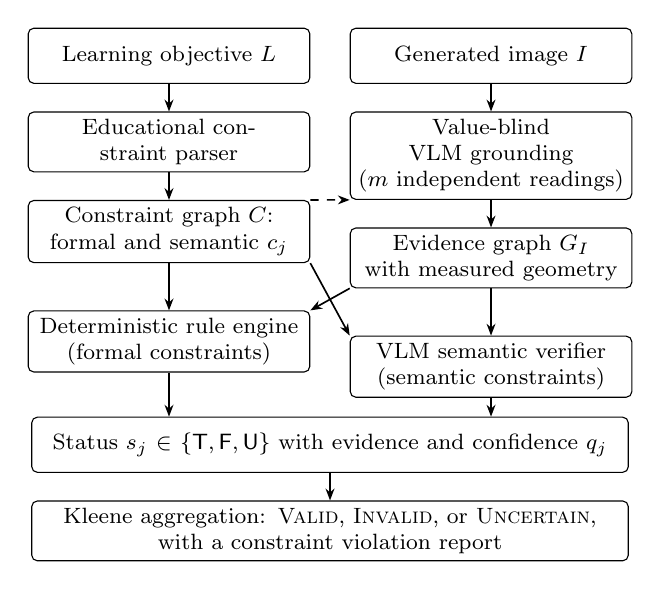
\begin{tikzpicture}[
  font=\footnotesize, node distance=3.5mm and 5mm,
  box/.style={draw, rounded corners=2pt, align=center, inner sep=2.5pt,
    minimum height=7mm, text width=34mm},
  wide/.style={box, text width=74mm},
  arr/.style={-{Stealth[length=1.5mm]}, semithick}]
\node[box] (L) {Learning objective $L$};
\node[box, right=of L] (I) {Generated image $I$};
\node[box, below=of L] (P) {Educational constraint parser};
\node[box, below=of I] (G) {Value-blind VLM grounding\\($m$ independent readings)};
\node[box, below=of P] (C) {Constraint graph $C$:\\formal and semantic $c_j$};
\node[box, below=of G] (E) {Evidence graph $G_I$\\with measured geometry};
\node[box, below=6mm of C] (R) {Deterministic rule engine\\(formal constraints)};
\node[box, below=6mm of E] (S) {VLM semantic verifier\\(semantic constraints)};
\node[wide, below=4mm of $(R.south)!0.5!(S.south)$] (A) {Status $s_j\in\{\sT,\sF,\sU\}$ with evidence and confidence $q_j$};
\node[wide, below=of A] (V) {Kleene aggregation: \Valid{}, \Invalid{}, or \Uncertain{},\\with a constraint violation report};
\draw[arr] (L) -- (P);
\draw[arr] (P) -- (C);
\draw[arr] (I) -- (G);
\draw[arr] (G) -- (E);
\draw[arr, dashed] (C.north east) -- (G.south west);
\draw[arr] (C) -- (R);
\draw[arr] (E) -- (S);
\draw[arr] (C.south east) -- (S.north west);
\draw[arr] (E.south west) -- (R.north east);
\draw[arr] (R.south) -- (R.south |- A.north);
\draw[arr] (S.south) -- (S.south |- A.north);
\draw[arr] (A) -- (V);
\end{tikzpicture}
\caption{EduAssetVerify. The grounding VLM receives only the vocabulary of the constraints (dashed arrow), never their target values. Rules decide the formal constraints from the evidence graph, a semantic verifier decides the rest, and an asset is accepted only if every constraint is verified.}
\label{fig:overview}
\end{figure}

\subsection{Educational Constraint Parser}\label{sec:parser}
The parser takes the learning objective and any asset requirements as text and returns a constraint graph whose nodes are entities (the whole, its parts, object sets) and constraints, with edges linking each constraint to the entities it mentions. It extracts the required concepts, maps them to schema constraints, identifies the required objects and relations, and checks the numeric constraints jointly for satisfiability, so that contradictory requirements are reported instead of verified. Two regimes are evaluated separately. With \emph{gold constraints}, authored alongside each benchmark template, the experiment isolates perception and verification. With \emph{extracted constraints}, produced by a language model from $L$, it measures the full pipeline, and extraction itself is scored against the gold set. Keeping the regimes apart prevents an extraction error from being reported as an image-verification error.

\subsection{Value-Blind Visual Grounding}\label{sec:grounding}
A VLM converts the image into an evidence graph
\begin{equation}
G_I=(O_I,R_I,A_I),\label{eq:evidence}
\end{equation}
where $O_I$ is the set of detected objects and regions, each with a category and a bounding region; $R_I$ holds the spatial and semantic relations between them; and $A_I$ holds their attributes, such as color, shading, text labels, and area. Four choices make $G_I$ evidence rather than opinion.

\emph{The prompt is value-blind.} It lists the entity and attribute vocabulary of $C$ (for example, \emph{whole}, \emph{part}, \emph{colored}, \emph{apple}) but none of the operators or target values. A model asked to confirm that four equal parts are present can agree without looking; a model asked to list the parts and mark the colored ones has to look.

\emph{The answer space is open and global.} Counts are returned as object lists rather than yes/no answers, and categories are drawn from a vocabulary that covers the whole domain, including distractors. A per-item candidate list that contains little besides the right answer makes every item trivially answerable, a degenerate setting that inflated every score in the game-asset study~\cite{anon2026legibility}.

\emph{Geometry is measured, not estimated.} Because VLMs misjudge precise geometry~\cite{rahmanzadehgervi2024blind}, areas and reflection overlaps are computed by deterministic measurement operators inside the regions that the VLM localizes, using color-connected components for flat renders and promptable segmentation~\cite{kirillov2023sam} for raster art. Every attribute records whether it was read by the VLM or measured.

\emph{Readings are repeated.} Grounding runs $m=3$ times independently, and Section~\ref{sec:abstain} turns disagreement between readings into uncertainty. Throughout, grounding sees only pixels: it never receives the renderer's hidden parameters, file names, or image metadata (Section~\ref{sec:construction}).

\subsection{Hybrid Constraint Verification}\label{sec:verify}
Each constraint $c_j$ receives a status $s_j\in\{\sT,\sF,\sU\}$: satisfied, violated, or undetermined.

\emph{Deterministic verification} handles the formal constraints: exact object counts, fraction and ratio values, spatial relations, geometric consistency, and logical combinations. Each checker states its preconditions, and a measured quantity whose deviation from its required value is $d_j$ receives
\begin{equation}
s_j=\begin{cases}\sT, & d_j\le\epsilon_j^{\sT},\\ \sF, & d_j\ge\epsilon_j^{\sF},\\ \sU, & \text{otherwise},\end{cases}\label{eq:zones}
\end{equation}
with tolerances $\epsilon_j^{\sT}<\epsilon_j^{\sF}$ fixed on the development split. Count checks compare the size of the matching object set with the target, and spatial checks compare region centroids with a margin proportional to object size. When a precondition fails, for example when the parts needed for an area check cannot be segmented, the status is $\sU$.

\emph{VLM semantic verification} handles the constraints that resist formalization: semantic correctness, object-category consistency, grounding of the educational concept, and visually ambiguous relations. Wherever possible, each is posed as an open question about specific nodes of $G_I$, such as what a label reads or which category an object belongs to, asked $m$ times, and the answers are compared with the target by the rule engine; only judgments that cannot be phrased this way, such as whether the image as a whole conveys the concept, are asked as yes/no questions.

The division of labor is strict. The rule engine decides only constraints for which the evidence is sufficient, and the semantic verifier never overrides a measured quantity. Insufficient evidence yields $\sU$ rather than a guess presented as a formal guarantee.

\subsection{Violation Detection and Localization}\label{sec:aggregate}
With the order $\sF<\sU<\sT$, the verdict is the strong Kleene conjunction of all constraint statuses:
\begin{equation}
V(I,C)=\begin{cases}\Valid, & \min_j s_j=\sT,\\ \Invalid, & \min_j s_j=\sF,\\ \Uncertain, & \text{otherwise}.\end{cases}\label{eq:verdict}
\end{equation}
One well-evidenced violation suffices to reject an asset, whereas acceptance requires every constraint to be positively verified. The asymmetry is deliberate, because accepting an asset that teaches the wrong concept costs more than sending a correct one to review. For each constraint, the report records its identifier, status, supporting evidence (graph nodes and measured values), violation type, affected object or region, and confidence. An unequal partition, for instance, is reported as \cn{equal\_area} $=\sF$, witnessed by the upper-right part, whose area deviation exceeds $\epsilon^{\sF}$ in all three readings.

\subsection{Verification Confidence and Abstention}\label{sec:abstain}
The confidence $q_j$ of a status averages an agreement weight over the $m$ readings. A reading that disagrees with the majority status has weight 0 and one that agrees has weight 1, except that for measured quantities an agreeing reading is weighted by its distance to the nearest threshold in \eqref{eq:zones}, relative to a fixed margin and capped at 1. A status is kept only if $q_j\ge\tau$ and is otherwise replaced by $\sU$, so that disagreement between readings, or between verifiers, surfaces as uncertainty and is recorded in the report; the verdict then follows from \eqref{eq:verdict}. The threshold $\tau$ thus controls false acceptance. Sweeping it traces a risk--coverage curve~\cite{geifman2017selective}, which we report in full rather than at a single operating point.

\section{Counterfactual Educational Asset Benchmark}\label{sec:benchmark}

\subsection{Design Principles}
The benchmark follows five principles: 1) ground truth that is verified programmatically, 2) controlled counterfactual pairs, 3) multiple educational domains, 4) visual diversity, and 5) test conditions unseen during development.

\subsection{Educational Task Categories}
\emph{Task A, fraction understanding,} covers equal partition, colored fractions, fraction comparison, and part-to-whole representation. \emph{Task B, object counting and classification,} covers exact counts, category-based counts, group comparison, and distractor objects. \emph{Task C, spatial reasoning,} covers left and right, above and below, rotation, reflection, symmetry, and relative position.

\subsection{Counterfactual Error Generation}
Each violated asset is derived from a correct one by a single controlled change,
\begin{equation}
I^{-}=T_k(I^{+}),\label{eq:cf}
\end{equation}
where $T_k$ is the $k$th error operator: missing object, extra object, incorrect proportion, incorrect label, spatial relation reversal, broken symmetry, or semantic mismatch (Fig.~\ref{fig:pairs}). The benchmark consists of pairs
\begin{equation}
D=\{(I^{+},I^{-},C,y^{+},y^{-})\},\label{eq:pairs}
\end{equation}
in which both images share the constraint set $C$, with $y^{+}=\Valid$ and $y^{-}=\Invalid$. Operators act on the scene specification rather than on pixels, and an assertion re-evaluates $C$ on both specifications: exactly the targeted constraint must change status, and every other constraint must keep its status. This single-variable property is what makes a pair diagnostic. Geometric perturbations change the affected quantity by at least a minimum $\delta_{\min}$ fixed before any verifier is run, and correct assets are exact by construction, so no label depends on measurement noise.

\begin{figure}[t]
\centering
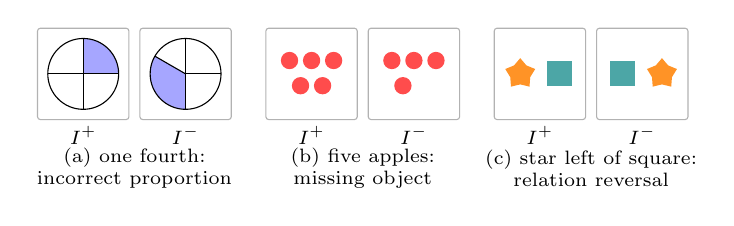
\begin{tikzpicture}[font=\scriptsize]
\foreach \x in {0,1.3,2.9,4.2,5.8,7.1}
  \draw[gray!60, rounded corners=1pt] (\x-0.58,-0.58) rectangle (\x+0.58,0.58);
\begin{scope}
  \fill[blue!35] (0,0) -- (0:0.45) arc (0:90:0.45) -- cycle;
  \draw (0,0) circle (0.45);
  \foreach \a in {0,90,180,270} \draw (0,0) -- (\a:0.45);
\end{scope}
\begin{scope}[xshift=1.3cm]
  \fill[blue!35] (0,0) -- (150:0.45) arc (150:270:0.45) -- cycle;
  \draw (0,0) circle (0.45);
  \foreach \a in {0,90,150,270} \draw (0,0) -- (\a:0.45);
\end{scope}
\begin{scope}[xshift=2.9cm]
  \foreach \p in {(-0.28,0.17),(0,0.17),(0.28,0.17),(-0.14,-0.15),(0.14,-0.15)}
    \fill[red!70] \p circle (0.11);
\end{scope}
\begin{scope}[xshift=4.2cm]
  \foreach \p in {(-0.28,0.17),(0,0.17),(0.28,0.17),(-0.14,-0.15)}
    \fill[red!70] \p circle (0.11);
\end{scope}
\begin{scope}[xshift=5.8cm]
  \node[star, star points=5, fill=orange!85, minimum size=4mm, inner sep=0pt] at (-0.25,0) {};
  \node[fill=teal!70, minimum size=3.2mm, inner sep=0pt] at (0.25,0) {};
\end{scope}
\begin{scope}[xshift=7.1cm]
  \node[fill=teal!70, minimum size=3.2mm, inner sep=0pt] at (-0.25,0) {};
  \node[star, star points=5, fill=orange!85, minimum size=4mm, inner sep=0pt] at (0.25,0) {};
\end{scope}
\foreach \x/\t in {0/{$I^{+}$},1.3/{$I^{-}$},2.9/{$I^{+}$},4.2/{$I^{-}$},5.8/{$I^{+}$},7.1/{$I^{-}$}}
  \node at (\x,-0.78) {\t};
\node[align=center] at (0.65,-1.2) {(a) one fourth:\\incorrect proportion};
\node[align=center] at (3.55,-1.2) {(b) five apples:\\missing object};
\node[align=center] at (6.45,-1.2) {(c) star left of square:\\relation reversal};
\end{tikzpicture}
\caption{Counterfactual pairs. Each violated asset $I^{-}$ applies one error operator to a correct asset $I^{+}$ and keeps every other property, so the two images share one constraint set and differ in exactly one constraint.}
\label{fig:pairs}
\end{figure}

\subsection{Dataset Construction}\label{sec:construction}
Table~\ref{tab:data} gives the planned composition. Assets come from four sources: a procedural renderer in Python that emits scalable vector graphics (SVG) from scene specifications, controlled transformations of those specifications, raster variants restyled by image generation models, and an independent rule-based validation of every label. The validation applies the principle that an answer key must be checked before any verifier is asked a question~\cite{anon2026legibility}. A measurement script recomputes each label from the rendered pixels, through region areas and connected components, without reading the specification, and an item enters the benchmark only if the two labels agree. Leakage is controlled at the same point: images receive random identifiers and stripped metadata, the specification stays with the evaluator, and an assertion scans every prompt sent to a model for specification fields and labels.

\begin{table}[t]
\caption{Planned Benchmark Composition}
\label{tab:data}
\centering
\begin{tabular}{@{}lrrr@{}}
\toprule
Domain & Correct & Violated & Total \\
\midrule
Fraction understanding & 150 & 150 & 300 \\
Object counting & 150 & 150 & 300 \\
Spatial reasoning & 150 & 150 & 300 \\
\midrule
Total & 450 & 450 & 900 \\
\bottomrule
\end{tabular}
\par\smallskip
\parbox{\columnwidth}{\centering\footnotesize\pending{Planned sizes; replace with the counts of the generated benchmark.}}
\end{table}

\subsection{Data Splits and Generalization}
All variants of one source template stay in the same split, so that no variant of a test image is seen during development. No component is trained; the development split serves only to design prompts and to set the tolerances and the threshold~$\tau$. The test conditions are in-domain; unseen asset template; unseen error combination, in which two operators are composed in a way never seen during development; unseen visual style; and cross-generator, with raster variants from generation models not used during development. Outputs of real generators do not always come with a label that can be confirmed automatically. Such variants are re-validated independently, and those without a trustworthy label are excluded from the main accuracy and reported separately.

\section{Experimental Setup}\label{sec:setup}

\subsection{Research Questions}
The experiments address four research questions (RQs).
\textbf{RQ1:} Does constraint-grounded verification outperform conventional VLM-based judging in detecting educational visual errors?
\textbf{RQ2:} Can EduAssetVerify correctly localize constraint violations?
\textbf{RQ3:} Does the framework generalize across educational tasks, visual styles, and generation models?
\textbf{RQ4:} What is the trade-off between verification accuracy, abstention, latency, and computational cost?

\subsection{Baseline Methods}
Table~\ref{tab:baselines} lists the six compared methods. All VLM-based methods use the same backbones, image resolution, and objective and constraint information, so that differences reflect the verification strategy rather than model capability. The similarity baseline thresholds CLIPScore~\cite{hessel2021clipscore} on the development split. The rule-only validator receives the same evidence graph as EduAssetVerify but has neither the semantic verifier nor abstention, and it maps undetermined statuses to \Invalid.

\begin{table}[t]
\caption{Compared Verification Methods}
\label{tab:baselines}
\centering
\begin{tabular}{@{}p{0.36\columnwidth}p{0.58\columnwidth}@{}}
\toprule
Method & Description \\
\midrule
Text--image similarity & CLIPScore between image and objective, thresholded \\
VLM direct judge & Asks the VLM whether the image is correct \\
VLM chain-of-thought (CoT) judge & Step-by-step visual reasoning, then a verdict \\
VLM structured judge & The VLM checks each constraint of $C$ in turn \\
Rule-only validator & Rules applied to the grounded evidence graph \\
EduAssetVerify & Value-blind grounding, hybrid verification, abstention \\
\bottomrule
\end{tabular}
\end{table}

\subsection{Evaluation Metrics}
\emph{Error detection.} \Invalid{} is the positive class. Precision, recall, and F1 are computed over answered items. The false acceptance rate (FAR) is the fraction of violated assets judged \Valid, and the false rejection rate (FRR) is the fraction of correct assets judged \Invalid. Both are computed over all items, so that abstaining never counts as acceptance.

\emph{Constraint level.} Constraint satisfaction accuracy compares each status with ground truth, violation type accuracy checks the inferred error operator, and localization accuracy counts a reported region as correct when its intersection over union with the perturbed region is at least 0.5.

\emph{Counterfactual.} Pairwise discrimination accuracy is the fraction of pairs with $V(I^{+})=\Valid$ and $V(I^{-})=\Invalid$; counterfactual consistency is the fraction of violated assets for which the reported violation is the perturbed constraint; and style invariance is the fraction of style-transformed assets whose verdict is unchanged.

\emph{Reliability and efficiency.} We report the abstention rate, the risk--coverage curve and the area under it, latency, input and output tokens, and the estimated cost per asset.

\subsection{Measurement Protocol and Guards}\label{sec:guards}
Before any of its numbers is reported, each VLM backbone, in every role, must pass a five-check validity battery adapted from the game-asset study~\cite{anon2026legibility}: 1) protocol compliance, meaning that every output parses against the schema; 2) test--retest agreement on repeated identical queries; 3) invariance to permuting answer options and vocabulary order; 4) a blank-image control, under which grounding must return no objects and judges must fall to chance; and 5) accuracy above a constant-majority predictor. Every configuration is then run in three independent evaluation passes, separate from the $m$ readings inside EduAssetVerify, and reported as mean $\pm$ standard deviation (sd). A difference is claimed only if it exceeds two standard errors and holds under every backbone. Table~\ref{tab:guards} lists the failure modes that the protocol guards against. Each guard is an executable assertion in the evaluation code rather than a written convention.

\begin{table}[t]
\caption{Failure Modes of Model-Judged Evaluation and Their Guards}
\label{tab:guards}
\centering
\begin{tabular}{@{}p{0.40\columnwidth}p{0.54\columnwidth}@{}}
\toprule
Failure mode & Executable guard \\
\midrule
API or parsing faults counted as wrong answers & Validity battery before scoring; unparsable outputs reported, never scored \\
Single-pass noise as large as the effects & Three passes per configuration; no per-cell number from fewer \\
Degenerate answer space & Value-blind, open-ended grounding; global vocabulary asserted to be much larger than any per-item candidate set \\
Abstention scored as error & Abstention, FAR, and FRR reported separately and asserted to be distinguishable \\
Answer leakage into prompts & No specification field or label in any prompt; random file names \\
Structure manufactured by small samples & Minimum items per cell; rank statistics only over five or more items \\
Judge from the generator's model family & Backbones from at least two model families; every claim must hold under each \\
Near-tautological measurement on clean renders & Clean renders reported separately from styled and generated images \\
\bottomrule
\end{tabular}
\end{table}

\subsection{Implementation Details}
\emph{Models:} \pending{VLM backbones with exact versions, from at least two model families; the language model used for constraint extraction; the image models used for the raster variants.} \emph{Prompts:} the templates of the judges, the constraint parser, and grounding are released with the code. \emph{Images:} rendered at \pending{resolution} pixels. \emph{Constraints and rules:} constraints are stored in a JSON schema that follows Section~\ref{sec:formulation}; \pending{rule engine implementation}. \emph{Runs:} three passes per configuration at \pending{sampling settings}; benchmark generation uses fixed random seeds, and the released code rebuilds every image from them. \emph{Hardware:} \pending{evaluation hardware}.

\section{Results and Analysis}\label{sec:results}

\pending{This section is filled from the experiment outputs once they exist. Every cell marked -- is a placeholder, and no number in this section is written by hand.}

\subsection{Overall Verification Performance}
Table~\ref{tab:main} compares all methods on error detection and answers RQ1. \pending{Findings.}

\begin{table*}[t]
\caption{Educational Constraint Violation Detection (RQ1)}
\label{tab:main}
\centering
\begin{tabular*}{\textwidth}{@{\extracolsep{\fill}}lccccccc@{}}
\toprule
Method & Precision & Recall & F1 & FAR $\downarrow$ & FRR $\downarrow$ & Abstention & AURC $\downarrow$ \\
\midrule
Text--image similarity & \tbd & \tbd & \tbd & \tbd & \tbd & \tbd & \tbd \\
VLM direct judge & \tbd & \tbd & \tbd & \tbd & \tbd & \tbd & \tbd \\
VLM CoT judge & \tbd & \tbd & \tbd & \tbd & \tbd & \tbd & \tbd \\
VLM structured judge & \tbd & \tbd & \tbd & \tbd & \tbd & \tbd & \tbd \\
Rule-only validator & \tbd & \tbd & \tbd & \tbd & \tbd & \tbd & \tbd \\
EduAssetVerify & \tbd & \tbd & \tbd & \tbd & \tbd & \tbd & \tbd \\
\bottomrule
\end{tabular*}
\par\smallskip
\parbox{\textwidth}{\footnotesize Mean $\pm$ sd over three passes. Precision, recall, and F1 over answered items; FAR, FRR, and abstention over all items; AURC: area under the risk--coverage curve.}
\end{table*}

\subsection{Performance across Educational Domains}
Table~\ref{tab:domain} breaks detection down by domain, to separate the errors that deterministic rules handle from those that need VLM semantics. \pending{Findings, including which constraint types each verifier handles.}

\begin{table}[t]
\caption{F1 and FAR by Educational Domain}
\label{tab:domain}
\centering
\begin{tabular}{@{}lcccccc@{}}
\toprule
& \multicolumn{2}{c}{Fraction} & \multicolumn{2}{c}{Counting} & \multicolumn{2}{c}{Spatial} \\
\cmidrule(lr){2-3}\cmidrule(lr){4-5}\cmidrule(l){6-7}
Method & F1 & FAR & F1 & FAR & F1 & FAR \\
\midrule
Direct judge & \tbd & \tbd & \tbd & \tbd & \tbd & \tbd \\
Structured judge & \tbd & \tbd & \tbd & \tbd & \tbd & \tbd \\
Rule-only & \tbd & \tbd & \tbd & \tbd & \tbd & \tbd \\
EduAssetVerify & \tbd & \tbd & \tbd & \tbd & \tbd & \tbd \\
\bottomrule
\end{tabular}
\end{table}

\subsection{Counterfactual Robustness}
Table~\ref{tab:cf} reports pairwise discrimination accuracy under each test condition, together with style invariance, and answers RQ3. \pending{Findings.}

\begin{table}[t]
\caption{Counterfactual Pair Evaluation (RQ3)}
\label{tab:cf}
\centering
\begin{tabular}{@{}lcccc@{}}
\toprule
Condition & Direct & Structured & Rule-only & Ours \\
\midrule
In-domain & \tbd & \tbd & \tbd & \tbd \\
Unseen template & \tbd & \tbd & \tbd & \tbd \\
Unseen error combination & \tbd & \tbd & \tbd & \tbd \\
Unseen visual style & \tbd & \tbd & \tbd & \tbd \\
Cross-generator & \tbd & \tbd & \tbd & \tbd \\
\midrule
Style invariance & \tbd & \tbd & \tbd & \tbd \\
\bottomrule
\end{tabular}
\end{table}

\subsection{Ablation Study}
Each configuration in Table~\ref{tab:ablation} removes one component and otherwise matches the full method, and an assertion in the evaluation code enforces the single difference. Without the rule engine, the VLM decides each formal constraint from the evidence graph; without structured grounding, the rules receive per-constraint yes/no answers from the VLM instead of the graph; without semantic verification, semantic constraints remain undetermined; and without abstention, $\tau=0$ and undetermined statuses map to \Invalid. The table also reports localization accuracy, which answers RQ2. \pending{Findings.}

\begin{table}[t]
\caption{Component Ablation (RQ2)}
\label{tab:ablation}
\centering
\begin{tabular}{@{}lcccc@{}}
\toprule
Configuration & F1 & FAR $\downarrow$ & Abstention & Localization \\
\midrule
Full EduAssetVerify & \tbd & \tbd & \tbd & \tbd \\
w/o rule engine & \tbd & \tbd & \tbd & \tbd \\
w/o structured grounding & \tbd & \tbd & \tbd & \tbd \\
w/o semantic verification & \tbd & \tbd & \tbd & \tbd \\
w/o abstention & \tbd & \tbd & \tbd & \tbd \\
\bottomrule
\end{tabular}
\end{table}

\subsection{Qualitative Error Analysis}
Fig.~\ref{fig:qual} shows correctly accepted, correctly rejected, falsely accepted, falsely rejected, and uncertain assets, each with its constraints, the verifier's report, and the ground truth. \pending{Discussion of the failure cases.}

\begin{figure}[t]
\centering
\fbox{\parbox[c][20mm][c]{0.92\columnwidth}{\centering\pending{Examples from the experiments: accepted, rejected, falsely accepted, falsely rejected, and uncertain assets, each with constraints, verifier report, and ground truth.}}}
\caption{Example verification results. \pending{Caption written with the figure.}}
\label{fig:qual}
\end{figure}

\subsection{Computational Efficiency}
Table~\ref{tab:cost} reports the cost of each method and answers RQ4 together with the risk--coverage results. \pending{Findings.}

\begin{table}[t]
\caption{Verification Cost and Latency (RQ4)}
\label{tab:cost}
\centering
\begin{tabular*}{\columnwidth}{@{\extracolsep{\fill}}lcccc@{}}
\toprule
Method & Time (s) & VLM calls & Tokens in/out & USD/1k \\
\midrule
Text--image sim. & \tbd & \tbd & \tbd & \tbd \\
Direct judge & \tbd & \tbd & \tbd & \tbd \\
CoT judge & \tbd & \tbd & \tbd & \tbd \\
Structured judge & \tbd & \tbd & \tbd & \tbd \\
Rule-only & \tbd & \tbd & \tbd & \tbd \\
EduAssetVerify & \tbd & \tbd & \tbd & \tbd \\
\bottomrule
\end{tabular*}
\par\smallskip
\parbox{\columnwidth}{\footnotesize Time and VLM calls per asset; cost per 1{,}000 assets at list prices on the run date.}
\end{table}

\section{Discussion}

\subsection{Implications for Generative AI in Education}
Constraint-grounded verification fits the point in an asset pipeline where generated material is accepted or sent back. Because acceptance requires positive evidence for every constraint, the verifier can serve as a quality gate for automated material production, and its abstentions define the review queue for teachers or designers. In the game-asset study, a critic loop changed review load rather than the property it was meant to improve~\cite{anon2026legibility}; the same distinction applies here, so the abstention rate is a cost to report rather than to hide. More broadly, separating perception from judgment offers a route to trustworthy multimodal verification wherever requirements can be stated explicitly.

\subsection{Advantages of Constraint-Grounded Verification}
By construction, the framework separates aesthetic quality from instructional correctness, turns a free-form visual judgment into structured evidence that can be inspected, makes every rejection reproducible from its report, and lets evaluation proceed with little human involvement, since benchmark labels come from the renderer rather than from raters. Whether these properties translate into better detection is the empirical question of Section~\ref{sec:results}.

\subsection{Limitations}
This work does not measure learning outcomes and makes no claim about learners' understanding or achievement. It covers only concepts whose correctness can be formalized as constraints, and many qualities of good teaching material, such as clarity or cultural fit, cannot be fully decided by program rules. Perception errors of the VLM still propagate into rule checks; repetition and abstention limit their effect but do not remove it. The benchmark is largely synthetic, which leaves a domain gap to real educational content. Finally, results depend on specific model versions, which change over time, so we report the versions and release the evaluation code for re-running.

\subsection{Future Work}
Next steps include more complex concepts and diagrams, verification of multimodal content that mixes text, images, and interaction, assessment inside interactive learning games, automatic repair driven by the violation report, and deployment studies with teachers in real courses.

\section{Conclusion}
We presented EduAssetVerify, a constraint-grounded framework for verifying AI-generated visual assets for education. It contributes a structured representation of educational constraints, a verification method that combines value-blind VLM grounding with deterministic rules and abstention, and a reproducible counterfactual benchmark with programmatically verified labels, evaluated under a protocol that guards against known failure modes of model-judged evaluation. \pending{State which hypotheses the experiments supported or refuted, with the key numbers.} The framework applies to concepts that can be stated as constraints, and it makes no claim about learning outcomes, which require studies with learners.

\bibliographystyle{IEEEtran}
\bibliography{aaie2027}

\end{document}
